\documentclass[main.tex]{subfiles}
% 线性变换的定义和基本性质
\begin{document}
在本节我们考虑由一个向量空间到另一个向量空间的一种映射。我们限定,建立了映射的两个向量空间是在同一数域上的。

向量空间之间的映射不一定保留其运算规则,即$f\left(\alpha\mathbf{a}+\beta\mathbf{b}\right)\neq\alpha f\left(\mathbf{a}\right)+\beta f\left(\mathbf{b}\right)$。如果两个同类代数结构之间的映射保持这类代数结构的关系定义不变,则称这种映射为同态映射(homomorphism)。
\begin{example}
以下映射是否同态映射?
\begin{itemize}
    \item $f:\mathbb{R}\rightarrow\mathbb{R}:f\left(x\right)=x^2$
    \item $g:\mathbb{R}^2\rightarrow\mathbb{R}:g\left(x,y\right)=x^2+y^2-4$
    \item $F:\mathbb{R}^2\rightarrow\mathbb{C}:F\left(x,y\right)=U\left(x,y\right)+iV\left(x,y\right),U,V:\mathbb{R}^2\rightarrow\mathbb{R}$
    \item $T:\mathbb{R}\rightarrow\mathbb{R}^2:T\left(t\right)=\left(t+3,2t-5\right)$
    \item 一个点粒子在空间中的运动可视为一个映射$M:\left[a,b\right]\rightarrow\mathbb{R}^3$,具体定义为对每一$t\in\left[a,b\right],M\left(t\right)=\left(x\left(t\right),y\left(t\right),z\left(t\right)\right)$,其中$x\left(t\right),y\left(t\right),z\left(t\right)$是$t$的实值函数。如果视$t$为时间,则$M\left(t\right)$描述了粒子的运动轨迹,$a$和$b$是运动的起始和终止时间。
\end{itemize}
\end{example}

\begin{definition}[线性变换]\label{def:II.4.1}
设$\mathcal{V}$和$\mathcal{W}$是$\mathbb{F}$上的向量空间。如果从$\mathcal{V}$到$\mathcal{W}$的映射$T:\mathcal{V}\rightarrow\mathcal{W}$满足
\[T\left(\alpha\mathbf{a}+\beta\mathbf{b}\right)=\alpha T\left(\mathbf{a}\right)+\beta T\left(\mathbf{b}\right)\]
则称$T$是从$\mathcal{V}$到$\mathcal{W}$的线性变换(linear transformation),常写成算符的形式:$T\left(\mathbf{a}\right)=\mathbf{Ta}$。如果两个线性变换$\mathbf{T}:\mathcal{V}\rightarrow\mathcal{W}$和$\mathbf{U}:\mathcal{V}\rightarrow\mathcal{W}$满足$\mathbf{Ta}=\mathbf{Ua}\forall\mathbf{a}\in\mathcal{V}$则称这两个线性变换相等,$\mathbf{U}=\mathbf{T}$。零变换$\mathbf{T}_0:\mathcal{V}\rightarrow\mathcal{W}$定义为$\mathbf{T}_0\mathbf{a}=\mathbf{0}_\mathcal{W}\forall\mathbf{a}\in\mathcal{V}$,其中$\mathbf{0}_\mathcal{W}\in\mathcal{W}$表示$\mathcal{W}$中的零向量\footnote{此处要注意区分不同向量空间中的零向量。}。\footnote{我们可以说线性变换就是向量空间之间的同态映射。}
\end{definition}

易验,任何一个线性变换都总把零向量映射为零向量。

易验两个向量空间之间的恒等映射是$\mathcal{V}$到其自身的线性变换$\mathbf{I}_\mathcal{V}:\mathcal{V}\rightarrow\mathcal{V},\mathbf{I}_\mathcal{V}\mathbf{a}=\mathbf{a}\forall\mathbf{a}\in\mathcal{V}$又可称为恒等线性变换。

正如由定义\ref{def:II.2.1}定义的向量那般,定义\ref{def:II.4.1}定义的线性变换也是抽象概念。例\ref{exp:II.2.1}中的向量空间上都可以建立线性变换。

\begin{example}\label{exp:II.4.2}
验证以下是例\ref{exp:II.2.1}中的$\mathcal{C}^\infty\left(a,b\right)$上的线性变换。
\begin{enumerate}
    \item 一阶导数映射$D:\mathcal{C}^\infty\left(a,b\right)\rightarrow\mathcal{C}^\infty\left(a,b\right),Df\left(x\right)=f^\prime\left(x\right),\forall f\in\mathcal{C}^\infty\left(a,b\right)$
    \item 积分上限函数映射$T:\mathcal{C}^\infty\left(a,b\right)\rightarrow\mathcal{C}^\infty\left(a,b\right),Tf\left(x\right)=\int_{0}^xf\left(x^\prime\right)dx^\prime,\forall f\in\mathcal{C}^\infty\left(a,b\right)$
    \item $F:\mathcal{C}^\infty\left(a,b\right)\rightarrow\mathcal{C}^\infty\left(a,b\right),Ff\left(x\right)=\sin\left(x\right)f\left(x\right),\forall f\in\mathcal{C}^\infty\left(a,b\right)$
\end{enumerate}
\end{example}

\begin{theorem}\label{thm:II.4.1}
设$\mathcal{V}$、$\mathcal{W}$是$\mathbb{F}$上的向量空间,$\mathbf{T}$、$\mathbf{U}$是从$\mathcal{V}$到$\mathcal{W}$的线性变换。若定义
\[\left(\mathbf{T}+\mathbf{U}\right)\mathbf{a}=\mathbf{Ta}+\mathbf{Ua},\forall\mathbf{a}\in\mathcal{V}\]
\[\left(\alpha\mathbf{T}\right)\mathbf{a}=\alpha\left(\mathbf{Ta}\right),\forall\alpha\in\mathbb{F}\]
则$\left(\mathbf{T}+\mathbf{U}\right)$和$\alpha\mathbf{T}$也是从$\mathcal{V}$到$\mathcal{W}$的线性变换。
\end{theorem}
\begin{proof}
分别用$\mathbf{T}+\mathbf{U}$和$\alpha\mathbf{T}$作用于向量$\beta\mathbf{a}+\gamma\mathbf{b},\alpha,\beta\in\mathbb{F},\mathbf{a},\mathbf{b}\in\mathcal{V}$,使用向量空间的定义\ref{def:II.2.1}、线性变换的定义\ref{def:II.4.1}和本命题中的运算定义证明。略。
\end{proof}

上面这一定理,事实上使得线性变换本身也能形成一个向量空间,作为推论如下。

\begin{corollary}
给定数域$\mathbb{F}$上的两个向量空间$\mathcal{V},\mathcal{W}$,所有由$\mathcal{V}$到$\mathcal{W}$的线性变换的集合是一个数域$\mathbb{F}$上的向量空间,记为$\mathcal{L}\left(\mathcal{V},\mathcal{W}\right)$,零变换是该向量空间的零向量。
\end{corollary}
\begin{proof}
前一句由定理\ref{thm:II.4.1}易证。设$\mathbf{T}_0$是由$\mathcal{V}$到$\mathcal{W}$的零变换,对任一$\mathbf{T}\in\mathcal{L}\left(\mathcal{V},\mathcal{W}\right)$和$\mathbf{a}\in\mathcal{V}$,$\left(\mathbf{T}_0+\mathbf{T}\right)\mathbf{a}=\mathbf{T}_0\mathbf{a}+\mathbf{Ta}=\mathbf{0}_\mathcal{W}+\mathbf{Ta}=\mathbf{Ta}$,即$\mathbf{T}_0+\mathbf{T}=\mathbf{T}\forall\mathbf{T}\in\mathcal{L}\left(\mathcal{V},\mathcal{W}\right)$。
\end{proof}

线性变换的空间$\mathcal{L}\left(\mathcal{V},\mathcal{W}\right)$作为一个向量空间,拥有一切向量空间的一般性质。注意在记法$\mathcal{L}\left(\mathcal{V},\mathcal{W}\right)$中,括号表示有序对。我们在这里考察$\mathcal{L}\left(\mathcal{V},\mathcal{W}\right)$的基和维数。

\begin{lemma}\label{lem:II.4.1}
设$\mathcal{V}_N$是数域$\mathbb{F}$上的$N$维向量空间,$B_\mathcal{V}=\left\{\mathbf{e}_i\right\}_{i=1}^N$是$\mathcal{V}_N$的一组基,$\mathcal{W}$是同数域上的另一向量空间。对$\mathcal{W}$中给定的任意一组$N$个不同向量$\left\{\mathbf{b}_i\right\}_{i=1}^N\in\mathcal{W}$,有且只有一个线性变换$\mathbf{T}:\mathcal{V}_N\rightarrow\mathcal{W}$满足$\mathbf{Te}_i=\mathbf{b}_i,i=1,\cdots,N$。
\end{lemma}
\begin{proof}
存在性的证明,只需找出这一线性变换。任一$\mathbf{a}\in\mathcal{V}_N$可用基$B_\mathcal{V}$表示成
\[\mathbf{a}=\sum_{i=1}^N\alpha_i\mathbf{e}_i,\alpha_i\in\mathbb{F},i=1,\cdots,N\]
特别地,
\[\mathbf{e}_i=\sum_{j=1}^N\delta_{ij}\mathbf{e}_j,i=1,\cdots,N\]
定义映射$\mathbf{T}:\mathcal{V}_N\rightarrow\mathcal{W},\mathbf{Ta}\equiv\sum_{i=1}^N\alpha_i\mathbf{b}_i$,则易验$\mathbf{Te}_i=\mathbf{b}_i,i=1,\cdots,N$。我们还需验证映射$\mathbf{T}$是线性变换,按定义\ref{def:II.4.1}只需验证$T\left(\alpha\mathbf{a}+\beta\mathbf{b}\right)=\alpha\left(\mathbf{Ta}\right)+\beta\left(\mathbf{Tb}\right)$即可。给定任意$\mathbf{b}\in\mathcal{V}_N$和标量$\gamma\in\mathbb{F}$,其中$\mathbf{b}$可表示为$\mathbf{b}=\sum_{i=1}^N\beta_i\mathbf{e}_i$,且有
\[\gamma\mathbf{a}+\mathbf{b}=\sum_{i=1}^N\left(\gamma\alpha_i+\beta_i\right)\mathbf{e}_i\]
由$\mathbf{T}$的定义有
\begin{align}
\mathbf{T}\left(\gamma\mathbf{a}+\mathbf{b}\right)&=\sum_{i=1}^N\left(\gamma\alpha_i+\beta_i\right)\mathbf{b}_i\\
\gamma\left(\mathbf{Ta}\right)+\mathbf{Tb}&=\gamma\sum_{i=1}^N\alpha_i\mathbf{b}_i+\sum_{i=1}^N\beta_i\mathbf{b}_i\\
&=\sum_{i=1}^N\left(\gamma\alpha_i+\beta_i\right)\mathbf{b}_i
\end{align}
所以$\mathbf{T}\left(\gamma\mathbf{a}+\mathbf{b}\right)=\gamma\left(\mathbf{Ta}\right)+\mathbf{Tb}$对任意向量$\mathbf{a},\mathbf{b}\in\mathcal{V}_N$和标题$\gamma\in\mathbb{F}$均成立,即$\mathbf{T}$是一个线性变换。存在性证毕。

唯一性的证明,设另有一线性变换$\mathbf{U}:\mathcal{V}_N\rightarrow\mathcal{W}$也满足$\mathbf{Ue}_i=\mathbf{b}_i$,则对任一$\mathbf{a}\in\mathcal{V}_N$,
\[
\mathbf{Ua}=\mathbf{U}\left(\sum_{i=1}^N\alpha_i\mathbf{e}_i\right)=\sum_{i=1}^N\alpha_i\mathbf{Ue}_i=\sum_{i=1}^N\alpha_i\mathbf{b}_i\]
即$\mathbf{U}$就是$\mathbf{T}$。
\end{proof}

\begin{theorem}\label{thm:II.4.2}
若$\mathcal{V}_N,\mathcal{W}_M$分别为数域$\mathbb{F}$上的$N,M$维向量空间,则$\mathcal{L}\left(\mathcal{V}_N,\mathcal{W}_M\right)$的维数是$M\times N$。
\end{theorem}
\begin{proof}
证明的过和,相当于找出$\mathcal{L}\left(\mathcal{V}_N,\mathcal{W}_M\right)$的基。

设$B_\mathcal{V}=\left\{\mathbf{e}_i\right\}_{i=1}^N,B_\mathcal{W}=\left\{\mathbf{f}_j\right\}_{j=1}^M$分别为$\mathcal{V}_N,\mathcal{W}_M$的基。对于每一对整数$\left(p,q\right),1\leq p\leq N,1\leq q\leq M$,定义一个线性变换$\mathbf{E}^{pq}:\mathcal{V}_N\rightarrow\mathcal{W}_M$\footnote{这一线性变换与例\ref{exp:II.3.2}中的矩阵很类似,可以比较理解。},
\[
\mathbf{E}^{pq}\mathbf{e}_i=\left\{\begin{array}{cc}
    \mathbf{0}_\mathcal{W},&i\neq p  \\
     \mathbf{f}_q,&i=p 
\end{array}\right.
\]
给定任一线性变换$\mathbf{T}\in\mathcal{L}\left(\mathcal{V}_N,\mathcal{W}_M\right)$,且令
\[\mathbf{Te}_i=\sum_{q=1}^MA_{qi}\mathbf{f}_q\]
由引理\ref{lem:II.4.1},对$\left\{\mathbf{f}_j\right\}_{j=1}^M$,$\mathbf{T}$是唯一的。且上式中的$A_{qi}$就是向量$\mathbf{Te}_i$在有序基$B_\mathcal{W}$下的坐标。

下面我们证明$\mathbf{T}$能被$\left\{\mathbf{E}^{pq}\right\}$线性表出。定义$\mathbf{U}\in\mathcal{L}\left(\mathcal{V}_N,\mathcal{W}_M\right)$,$\mathbf{Ue}_i=\sum_p\sum_qA_{qp}\mathbf{E}^{pq}\mathbf{e}_i$,则
\begin{align*}
    \mathbf{Ue}_i&=\sum_p\sum_qA_{qp}\mathbf{E}^{pq}\mathbf{e}_i\\
    &=\sum_p\sum_qA_{qp}\delta_{ip}\mathbf{f}_q\\
    &=\sum_qA_{qi}\mathbf{f}_q\\
    &=\mathbf{Te}_i
\end{align*}
则可见$\mathbf{U}=\mathbf{T}$,同时有
\[\mathbf{T}=\sum_{p=1}^N\sum_{q=1}^MA_{qp}\mathbf{E}^{pq}\]
由于$\mathbf{T}$是$\mathcal{L}\left(\mathcal{V}_N,\mathcal{W}_M\right)$中的任意一个线性变换,故$\mathcal{L}\left(\mathcal{V}_N,\mathcal{W}_M\right)$是$\left\{\mathbf{E}^{pq}\right\}$的线性生成空间。由基的定义\ref{def:II.2.5},现在我们只需再证$\left\{\mathbf{E}^{pq}\right\}$是线性无关的,它们就是$\mathcal{L}\left(\mathcal{V}_N,\mathcal{W}_M\right)$的基了。按照线性无关的定义,设$\mathbf{T}$是零变换,由于$\left\{\mathbf{f}_j\right\}_{j=1}^M$是线性无关的,
\[\mathbf{T}=\mathbf{0}=\sum_{p=1}^N\sum_{q=1}^MA_{qp}\mathbf{E}^{pq}\Leftrightarrow\mathbf{Te}_i=\sum_q A_{qi}\mathbf{f}_q=\mathbf{0}_\mathcal{W}\Leftrightarrow A_{qi}=0\forall q=1,\cdots,M,i=1,\cdots,N\]
即$\left\{\mathbf{E}^{pq}\right\}$线性无关。故$\left\{\mathbf{E}^{pq}\right\}$是$\mathcal{L}\left(\mathcal{V}_N,\mathcal{W}_M\right)$的一组基,$\mathcal{L}\left(\mathcal{V}_N,\mathcal{W}_M\right)$的维数就是$M\times N$。
\end{proof}

注意,给定两个有限维向量空间$\mathcal{V},\mathcal{W}$,$\mathcal{L}\left(\mathcal{V},\mathcal{W}\right)$中的线性变换和$\mathcal{L}\left(\mathcal{W},\mathcal{V}\right)$中的线性变换是不同空间的元素,没有一般关系——虽然它们的维数无非只是$M\times N$和$N\times M$差别。在本讲义中我们会注意线性变换维数写法的顺序。

讨论完线性变换本身作为向量的性质,我们接下来考虑线性变换作为映射的性质:单射、满射、双射……。线性变换作为映射的性质与它所映射的两个向量空间的维数有关,这是线性代数最重要的定理之一,下面先给出这一定理。

\begin{definition}[零空间、零化度、秩]\label{def:II.4.2}
(如图\ref{fig:II.4.1}所示)设$\mathcal{V}$和$\mathcal{W}$是数域$\mathbb{F}$上的向量空间。线性变换$\mathbf{T}:\mathcal{V}\rightarrow\mathcal{W}$的零空间(null space)或核空间(kernel),记作$\mathrm{ker}\mathbf{T}$,是所有满足$\mathbf{Ta}=\mathbf{0}_\mathcal{W}$的向量$\mathbf{a}$的集合。零空间的维数称为该线性变换的零化度(nullity),记作$\mathrm{nullity}\mathbf{T}\equiv\mathrm{dim}\left(\mathrm{ker}\mathbf{T}\right)$。如果$\mathcal{V}$是有限维向量空间,则$\mathbf{T}$的秩(rank)是$\mathbf{T}$的值域的维数,记作$\mathrm{rank}\mathbf{T}\equiv\mathrm{dim}\left(\mathrm{ran}\mathbf{T}\right)$。特别地,如果$\mathrm{nullity}\mathbf{T}=0$,即$\mathbf{T}$的零空间只有零向量$\mathbf{0}_\mathcal{V}$一个元素,则称$\mathbf{T}$是非奇异的(non-singular)。
\end{definition}

\begin{figure}[htbp]
\centering
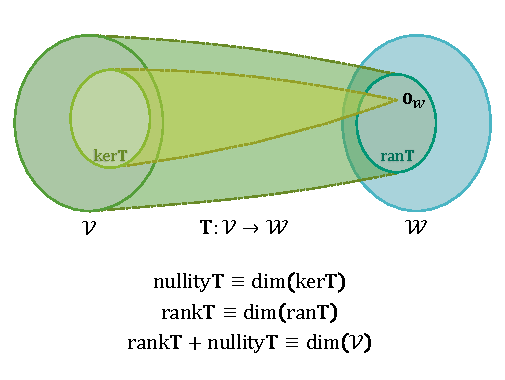
\includegraphics{images/II.4.1.pdf}
\caption{线性变换的零空间、值域、零化度和秩以及线性变换的维数定理表达式}
\label{fig:II.4.1}
\end{figure}

上述定义默认了两个易验事实的成立:$\mathrm{ker}\mathbf{T}$是$\mathcal{V}$的子空间,$\mathrm{ran}\mathbf{T}$是$\mathcal{W}$的子空间(否则不能直接谈它这两个子集的“维数”),证明从略\cite[\S7.3“2.线性变换的简单性质(4)”p.~177]{周胜林2012线性代数}。基于定义\ref{def:II.4.2}的概念,我们给出线性代数中非常重要的定理——线性变换的维数定理(\S7.3“2.线性变换的简单性质(5)”\cite[p.~178]{周胜林2012线性代数})。

\begin{theorem}[线性变换的维数定理]\label{thm:II.4.3}
设$\mathcal{V}$和$\mathcal{W}$是数域$\mathbb{F}$上的向量空间,其中$\mathcal{V}$是有限维向量空间,则对线性变换$\mathbf{T}:\mathcal{V}\rightarrow\mathcal{W}$有
\[
\mathrm{rank}\mathbf{T}+\mathrm{nullity}\mathbf{T}=\mathrm{dim}\mathcal{V}
\]
\end{theorem}
\begin{proof}
设$\mathrm{dim}\mathcal{V}=n$,$\mathrm{nullity}\mathbf{T}=\mathrm{dim}\left(\mathrm{ker}\mathbf{T}\right)=k$,$\left\{\mathbf{a}_1,\cdots,\mathbf{a}_k\right\}$是$\mathrm{ker}\mathbf{T}$的一组基。则可在$\mathcal{V}$中继续找到$\left\{\mathbf{a}_{k+1},\cdots,\mathbf{a}_{n}\right\}$与$\left\{\mathbf{a}_1,\cdots,\mathbf{a}_k\right\}$合并成线性无关向量组,从而成为$\mathcal{V}$的基。

由于$\left\{\mathbf{Ta}_1,\cdots,\mathbf{Ta}_n\right\}$线性生成$\mathbf{T}$的值域$\mathrm{ran}\mathbf{T}$(由线性变换性质易证),其中由于$\left\{\mathbf{a}_1,\cdots,\mathbf{a}_k\right\}\in\mathrm{ker}\mathbf{T}$,故有$\mathbf{Ta}_j=\mathbf{0}_\mathcal{W}\forall j\leq k$,所以实际上仅$\left\{\mathbf{Ta}_{k+1},\cdots,\mathbf{Ta}_n\right\}$就线性生成$\mathrm{ran}\mathbf{T}$了。我们进一步验证它们是线性无关的。设标量$\gamma_i$满足$\sum_{i=k+1}^n\gamma_i\mathbf{Ta}_i=\mathbf{0}_\mathcal{W}$,即
\[\mathbf{T}\left(\sum_{i=k+1}^n\gamma_i\mathbf{a}_i\right)=\mathbf{0}_\mathcal{W}\]
即$\sum_{i=k+1}^n\gamma_i\mathbf{a}_i\equiv\mathbf{a}\in\mathcal{N}$。向量$\mathbf{a}$在$\mathrm{ker}\mathbf{T}$的基$\left\{\mathbf{a}_1,\cdots,\mathbf{a}_k\right\}$下表示为$\mathbf{a}=\sum_{i=1}^k\alpha_i\mathbf{a}_i$。故
\[
\mathbf{a}=\sum_{i=1}^k\alpha_i\mathbf{a}_i=\sum_{j=k+1}^n\gamma_j\mathbf{a}_j
\]
由于$\left\{\mathbf{a}_1,\cdots,\mathbf{a}_n\right\}$是线性无关的,故有且只有$\alpha_1=\cdots=\alpha_k=\gamma_{k+1}=\cdots=\gamma_n=0$,即$\left\{\mathbf{Ta}_{k+1},\cdots,\mathbf{Ta}_n\right\}$是线性无关的。因此$\left\{\mathbf{Ta}_{k+1},\cdots,\mathbf{Ta}_n\right\}$是$\mathcal{W}$的基,即$\mathcal{W}$的维数是$n-k$,由定义\ref{def:II.4.2}即$\mathrm{rank}\mathbf{T}=n-k$。
\end{proof}

线性变换的维数定理是我们继续讨论线性变换的映射性质的重要定理。我们首先考虑一个线性变换是单射的情况。

\begin{theorem}\label{thm:II.4.4}
设$\mathcal{V},\mathcal{W}$是数域$\mathbb{F}$上的有限维向量空间,$\mathbf{T}:\mathcal{V}\rightarrow\mathcal{W}$是一个线性变换,则以下命题互相等价:
\begin{enumerate}
    \item $\mathbf{T}$是非奇异的;
    \item $\mathbf{T}$是单射;
    \item $\mathbf{T}$将$\mathcal{V}$中的任意一组线性无关向量组映射为$\mathcal{W}$的一组线性无关向量组;
    \item $\mathrm{rank}\mathbf{T}=\mathrm{dim}\mathcal{V}$。
\end{enumerate}
\end{theorem}
\begin{proof}
$1\Leftrightarrow 2$:设$\mathbf{T}$是非奇异的(即有$\mathbf{Ta}=\mathbf{0}_\mathcal{W}\Leftrightarrow\mathbf{a}=\mathbf{0}_\mathcal{V}\forall\mathbf{a}\in\mathcal{V}$),则对任意$\mathbf{a},\mathbf{b}\in\mathcal{V}$,$\mathbf{Ta}=\mathbf{Tb}\Leftrightarrow\mathbf{T}\left(\mathbf{a}-\mathbf{b}\right)=\mathbf{0}_\mathcal{W}\Leftrightarrow\mathbf{a}-\mathbf{b}=\mathbf{0}_\mathcal{V}\Leftrightarrow\mathbf{a}=\mathbf{b}$。

$1\Leftrightarrow 3$:设$\mathbf{T}$是非奇异的。令$S$是$\mathcal{V}$的一个线性无关向量组,如果向量$\mathbf{a}_1,\cdots,\mathbf{a}_k\in S$,则
\[
\sum_{i=1}^kc_i\left(\mathbf{Ta}_i\right)=\mathbf{0}_\mathcal{W}\Leftrightarrow\mathbf{T}\sum_{i=1}^kc_i\mathbf{a}_i=\mathbf{0}_\mathcal{W}\Leftrightarrow\sum_{i=1}^kc_i\mathbf{a}_i=\mathbf{0}_\mathcal{W}\Leftrightarrow c_i=0\forall i
\]
假设$\mathbf{T}$总把$\mathcal{V}$的一组线性无关向量映射为$\mathcal{W}$的一组线性无关向量,令$\mathbf{a}\neq\mathbf{0}_\mathcal{V}$是$\mathcal{V}$的一个非零向量,则只含$\mathbf{a}$的向量组$\left\{\mathbf{a}\right\}$是线性无关向量组,这时$\mathbf{Ta}$必不为$\mathbf{0}_\mathcal{W}$,因为单一个零向量的向量组是线性相关的,违反了假设。因此$\mathbf{T}$只能把$\mathbf{0}_\mathcal{V}$映射为$\mathbf{0}_\mathcal{W}$,即为非奇异的。

$1\Leftrightarrow 4$:由定理\ref{thm:II.4.3}可直接得到。
\end{proof}

定理\ref{thm:II.4.4}联系了线性变换的非奇异性与其单射性。下面的推论进一步说明,如果在此基础上再加上一个条件:$\mathrm{dim}\mathcal{V}=\mathrm{dim}\mathcal{W}$,那么$\mathbf{T}$要么是双射,要么是非单射非满射。

\begin{corollary}
设$\mathcal{V},\mathcal{W}$是数域$\mathbb{F}$上的有限维向量空间且$\mathrm{dim}\mathcal{V}=\mathrm{dim}\mathcal{W}$,$\mathbf{T}:\mathcal{V}\rightarrow\mathcal{W}$是一个线性变换,则以下命题相互等价:
\begin{enumerate}
    \item $\mathbf{T}$是单射;
    \item $\mathbf{T}$是满射;
    \item $\mathbf{T}$将$\mathcal{V}$中的任意一组基映射为$\mathcal{W}$的一组基;
\end{enumerate}
\end{corollary}
\begin{proof}
$1\Leftrightarrow 2$:设$n=\mathrm{dim}\mathcal{V}=\mathrm{dim}\mathcal{W}$,则由定理\ref{thm:II.2.1}的推论3、定理\ref{thm:II.4.3}和\ref{thm:II.4.4},$\mathbf{T}$是单射$\Leftrightarrow\mathrm{rank}\mathbf{T}=n=\mathrm{dim}\mathcal{W}\Leftrightarrow\mathrm{ran}\mathbf{T}=\mathcal{W}$。

$1\Leftrightarrow 3$:留作练习。
\end{proof}

由定理\ref{thm:II.1.7},作为双射的线性变换必存在唯一逆映射,那么这个逆映射会不会也是一个线性变换呢?答案是肯定的。

\begin{theorem}
设$\mathcal{V},\mathcal{W}$是数域$\mathbb{F}$上的向量空间,$\mathbf{T}:\mathcal{V}\rightarrow\mathcal{W}$是一个线性变换。如果$\mathbf{T}$可逆,则其逆映射$\mathbf{T}^{-1}$是一个由$\mathcal{W}$到$\mathcal{V}$的线性变换。
\end{theorem}
\begin{proof}
对任意$\mathbf{b}_1,\mathbf{b}_3\in\mathcal{W}$和$\gamma\in\mathbb{F}$,令$\mathbf{a}_i=\mathbf{T}^{-1}\mathbf{b}_i,i=1,2$,由于$\mathbf{T}$是线性变换,则有$\mathbf{T}\left(\gamma\mathbf{b}_1+\mathbf{b}_2\right)=\gamma\mathbf{Ta}_1+\mathbf{Ta}_2=\gamma\mathbf{b}_1+\mathbf{b}_2$。因此向量$\gamma\mathbf{a}_1+\mathbf{a}_2\in\mathcal{V}$就是向量$\gamma\mathbf{b}_1+\mathbf{b}_2\in\mathcal{W}$在映射$\mathbf{T}$下的原像,由逆映射性质有$\mathbf{T}^{-1}\left(\gamma\mathbf{b}_1+\mathbf{b}_2\right)=\gamma\mathbf{a}_1+\mathbf{a}_2=\gamma\left(\mathbf{T}^{-1}\mathbf{b}_1\right)+\mathbf{T}^{-1}\mathbf{b}_2$,即$\mathbf{T}^{-1}$满足线性变换定义的性质(对任意选取的$\mathbf{b}_1,\mathbf{b}_2,\gamma$均成立),故$\mathbf{T}^{-1}$是线性变换。
\end{proof}

双射(可逆)线性变换,经常称作“同构线性变换”(isomorphic linear transformation)。如果两个向量空间之间存在一个同构线性变换,则称这两个向量空间是同构(isomorphic)的。在\S\ref{sec:II.2}中我们了解了向量与其在给定某基下的坐标是一一对应的,且易证这一对应关系是一个同构线性变换。因此,事实上任一$n$维向量空间均与$n$维坐标空间$\mathbb{F}^n$同构。由于双射的可逆性具有传递性,即当$f:A\rightarrow B$是双射、$g:B\rightarrow C$是双射,则$g\circ f:A\rightarrow C$是双射,故所有同维数的向量空间之间相互同构。以下定理及其推论从一个不同的出发点证明了这上述的结论。

\begin{theorem}\label{thm:II.4.6}
数域$\mathbb{F}$上的两个向量空间同构当且仅当它们维数相等。
\end{theorem}
\begin{proof}
由“两个向量空间同构”的定义,需要证明两个维数相同的向量空间中存在一个双射线性变换。设$\mathcal{V}_N$、$\mathcal{W}_N$是数域$\mathbb{F}$上的两个$N$维向量空间。分别给定$\mathcal{V}_N,\mathcal{W}_N$的各一组有序基$B_\mathcal{V}=\left\{\mathbf{e}_i\right\}_{i=1}^N, B_\mathcal{W}=\left\{\mathbf{f}_i\right\}_{i=1}^N$,构建一个线性变换$\mathbf{T}:\mathcal{V}_N\rightarrow\mathcal{W}_N$,对$\mathcal{V}_N$中的任一向量$\mathbf{a}=\sum_{i=1}^N\alpha_i\mathbf{e}_i$,$\mathbf{Ta}=\sum_{i=1}^N\alpha_i\mathbf{f}_i$。易验$\mathbf{a}=\mathbf{0}_\mathcal{V}\Leftrightarrow\mathbf{Ta}=\mathbf{0}_\mathcal{W}$,即$\mathbf{T}$是单射。由定理\ref{thm:II.4.4}及其推论可知$\mathbf{T}$是双射。
\end{proof}

\begin{corollary}
任一数域$\mathbb{F}$上的$N$维向量空间均与$\mathbb{F}^N$同构
\end{corollary}

按照逆映射的性质,一个同构线性变换与其逆映射的复合映射是恒等映射。我们于是要问:两个线性变换形成的复合映射是线性变换吗?答案是肯定的。

\begin{theorem}\label{thm:II.4.7}
设$\mathcal{V},\mathcal{W},\mathcal{Z}$是数域$\mathbb{F}$上的向量空间,$\mathbf{T}:\mathcal{V}\rightarrow\mathcal{W},\mathbf{U}:\mathcal{W}\rightarrow\mathcal{Z}$是线性变换,则复合映射$\mathbf{U}\circ\mathbf{T}$(记为$\mathbf{UT}$)也是线性变换。
\end{theorem}
\begin{proof}
用$\mathbf{UT}$作用于$\gamma\mathbf{a}+\mathbf{b}$,其中$\mathbf{a},\mathbf{b}\in\mathcal{V},\gamma\in\mathbb{F}$是任意的,证明$\gamma\left(\mathbf{UT}\right)\mathbf{a}+\left(\mathbf{UT}\right)\mathbf{b}$即可,留作练习。
\end{proof}

由此定理易得推论:向量空间的恒等映射总是同构线性变换,称为恒等线性变换或恒等变换,记为$\mathbf{I}_\mathcal{V}$,其中$\mathcal{V}$是这个恒等变换所作用的向量空间。

\begin{example}
设$\mathcal{V},\mathcal{W}$是数域$\mathbb{F}$上的向量空间,$\mathbf{T}:\mathcal{V}\rightarrow\mathcal{W}$是同构线性变换。则$\mathbf{T}^{-1}\mathbf{T}=\mathbf{I}_\mathcal{V},\mathbf{TT}^{-1}=\mathbf{I}_\mathcal{W}$。
\end{example}

\begin{definition}[线性算符]\label{def:II.4.3}
设$\mathcal{V}$是数域$\mathbb{F}$上的向量空间,由$\mathcal{V}$到其自身的线性变换$\mathbf{T}:\mathcal{V}\rightarrow\mathcal{V}$称为线性算符(linear operator)。
\end{definition}

线性变换是向量空间之间的同态映射,故线性算符又可称为自同态(automorphic)线性变换。同态的双射叫同构映射(isomorphism),前面也提到过双射的线性变换叫同构线性变换,故双射的线性算符又称自同构(endomorphic)线性算符。由定理\ref{thm:II.4.4}的推论,线性算符要么是非单射非满射,要么是双射。也就是说,并非所有线性算符都是可逆映射,只有是双射(自同构)的线性算符才是可逆映射。自同构线性算符与其逆映射同属于同一个线性变换的空间$\mathcal{L}\left(\mathcal{V},\mathcal{V}\right)$(简写为$\mathcal{L}\left(\mathcal{V}\right)$)。

对于一般的线性变换,本节开头介绍了其作为向量的线性代数。现在我们可以通过复合变换的定义,为线性算符引入“乘法”的代数\footnote{代数(algebra)的定义此略,此处只强调,要成为代数的运算,其中一个必要条件是要具有封闭性。一般的线性变换的复合操作不满足此条件。}。此时恒等变换记号$\mathbf{I}$无需指明作用空间。

\begin{theorem}\label{thm:II.4.8}
设$\mathcal{V}$是数域$\mathbb{F}$上的向量空间,$\mathbf{U},\mathbf{T}_1,\mathbf{T}_2\in\mathcal{L}\left(\mathcal{V}\right)$,$\gamma\in\mathbb{F}$,则有:
\begin{enumerate}
    \item $\mathbf{IU}=\mathbf{UI}=\mathbf{U}$
    \item $\mathbf{U}\left(\mathbf{T}_1+\mathbf{T}_2\right)=\mathbf{UT}_1+\mathbf{UT}_2$,$\left(\mathbf{T}_1+\mathbf{T}_2\right)\mathbf{U}=\mathbf{T}_1\mathbf{U}+\mathbf{T}_2\mathbf{U}$
    \item $\gamma\mathbf{UT}_1=\left(\gamma\mathbf{U}\right)\mathbf{T}_1=\mathbf{U}\left(\gamma\mathbf{T}_1\right)$
\end{enumerate}
\begin{proof}
第1条由相关定义是易证的。

对任一向量$\mathbf{a}\in\mathcal{V}$,
\begin{align*}
    \left[\mathbf{U}\left(\mathbf{T}_1+\mathbf{T}_2\right)\right]\mathbf{a}&=\mathbf{U}\left[\left(\mathbf{T}_1+\mathbf{T}_2\right)\mathbf{a}\right]\quad\text{(由定理\ref{thm:II.4.1}中的定义)}\\
    &=\mathbf{U}\left(\mathbf{T}_1\mathbf{a}+\mathbf{T}_2\mathbf{a}\right)\quad\text{($\mathbf{U}$是线性变换)}\\
    &=\left(\mathbf{UT}_1\right)\mathbf{a}+\left(\mathbf{UT}_2\right)\mathbf{a}\quad\text{(由复合映射的定义)}
\end{align*}
故由两映射相等的定义,$\mathbf{U}\left(\mathbf{T}_1+\mathbf{T}_2\right)=\mathbf{UT}_1+\mathbf{UT}_2$。类似地,
\begin{align*}
    \left[\left(\mathbf{T}_1+\mathbf{T}_2\right)\mathbf{U}\right]\mathbf{a}&=\left(\mathbf{T}_1+\mathbf{T}_2\right)\left(\mathbf{Ua}\right)\quad\text{(由复合映射的定义)}\\
    &=\mathbf{T}_1\left(\mathbf{Ua}\right)+\mathbf{T}_2\left(\mathbf{Ua}\right)\quad\text{(由定理\ref{thm:II.4.1}中的定义)}\\
    &=\left(\mathbf{T}_1\mathbf{U}\right)\mathbf{a}+\left(\mathbf{T}_2\mathbf{U}\right)\mathbf{a}\quad\text{(由复合映射的定义)}
\end{align*}
故由两映射相等的定义,$\left(\mathbf{T}_1+\mathbf{T}_2\right)\mathbf{U}=\mathbf{T}_1\mathbf{U}+\mathbf{T}_2\mathbf{U}$,第2条证毕\footnote{我们留意到第2条的第一部分证明没有用到$\mathbf{T}_1$和$\mathbf{T}_2$是线性变换的条件,第二部分的证明连$\mathbf{U}$是线性变换的条件都没用到。}。第3条证明留作练习。
\end{proof}
\end{theorem}
\end{document}